\documentclass[paper=a4, fontsize = 12pt, DIV = calc, twoside=off, parskip=full, numbers=noenddot]{scrbook}
\usepackage[utf8]{inputenc}
\usepackage[ngerman]{babel}
\usepackage{blindtext}
\usepackage{microtype}
\usepackage{hyperref}
\usepackage{csquotes}
\usepackage{glossaries}
\usepackage{graphicx}
\usepackage{fancyref}
\usepackage{subcaption}
\usepackage{wrapfig}
\usepackage{float}
\usepackage{svg}
\makeglossaries
\newglossaryentry{airflow-code-editor}{
name = airflow-code-editor,
description = {Airflow-code-editor ist ein open-source Plugin (Apache-2.0 Lizenz) für Airflow, welches das programmierbasierte Editieren und Erstellen von DAGs in der Weboberfläche von Airflow ermöglicht. \nolinkurl{https://github.com/andreax79/airflow-code-editor}}
}

\newglossaryentry{AppBuilder}{ %Hier sollte noch mehr hin wahrscheinlich
name = \textit{AppBuilder},
description = Flask-AppBuilder ist ein Development-Framework welches auf Flask basiert. Es wird von
Airflow ab Version 2.0.0 für die Darstellung der Weboberfläche verwendet.
\nolinkurl{https://github.com/dpgaspar/Flask-AppBuilder}}

\newglossaryentry{Op}{ %Hier sollte noch mehr hin wahrscheinlich und was ist hier die Formale Definition hab mich dran versucht
name = Op,
description = Der Server Operator ist ein Nutzer welcher Schreibzugriff auf die grundlegende Konfiguration der Anwendung hat. Er ist somit in der Lage die Konfiguration der Serverstruktur der
Anwendung zu ändern.}

\newglossaryentry{Codemirror}{
name = Codemirror,
description = {Ist ein Editor zum Bearbeiten von Code in Webbrowsern welcher auf JavaScript basiert. 
Er ist open-source und wird steht unter der MIT-Lizenz. \nolinkurl{https://github.com/codemirror/CodeMirror}}
%\nolinkurl{https://github.com/codemirror/CodeMirror}
}

\newglossaryentry{Apache Airflow}{
name = Apache Airflow,
description ={Open-source Workflow Management Plattform für Workflows}
}

\title{{WAMS}\\
{\Large{Workflow Application for Material Sciences}}\\
{Entwurfsdokument}}
\author{Dominik Siebelt \and Max Umbach 
        \and Maxim Besser \and Isabel Kraft \and Fabian Zürker}
\date{Dezember 2021}

\begin{document}

\maketitle
\newpage
\setcounter{tocdepth}{1}
\tableofcontents
\newpage

\chapter{Einleitung}
WAMS baut auf der Basis von \Gls{Apache Airflow} auf und erweitert bzw. ändert die Standardkonfiguration von Airflow ab, sodass der geforderte Funktionsumfang erreicht wird.
Dafür bringt WAMS ein eigenes Plugin mit, das weitere Webansichten und Operatoren einfügt.
Diese Ergänzungen ermöglichen es WAMS mehr Funktionalität über die Weboberfläche anzubieten.

Dass WAMS Airflow als Basis nutzt und darauf aufbaut, ergibt folgende Vorteile:
\begin{itemize}
    \item Die Funktionalität von Airflow bleibt erhalten, sodass WAMS ebenso mit dem Ökosystem von Airflow interagieren kann.
    \item Updates von Airflow können ohne Anpassung des WAMS-Plugins übernommen werden.
    \item Weite Teile der Deployment-Logistik Airflows werden übernommen.
\end{itemize}
Jedoch liefert Airflow noch nicht gesamten Funktionsumfang der von WAMS gefordert wird. Wie der geforderte Funktionsumfang erreicht wird, wird im Folgenden beschrieben.

%
%Dies ermöglicht das Apache Airflow unabhängig von WAMS aktualisiert werden kann.
%Dies verbessert die Erweiterbarkeit von WAMS durch die Installation von Airflow Plugins.
%Dies ermöglicht das WAMS erweiterbar ist durch die Installation von Airflow Plugins.
%Dies ermöglicht eine Verwendung von der aktuellen Airflow Version selbst bei updates.

\section{Paketstruktur}

%WAMS besteht aus zwei Hauptbestandteilen. In diesen sind Klassen mit ähnlichen Funktionen 
%zusammengefasst.
WAMS kann grob in zwei Bestandteile aufgeteilt werden:
\begin{itemize}
    \item Eine Airflow-Instanz mit spezieller Konfiguration
    \item Das eigene Plugin, welches die Weboberfläche von Airflow erweitert
\end{itemize}

Airflow bietet für Plugins eine eigene Schnittstelle an, die von WAMS genutzt wird, um eigene 
Webansichten hinzuzufügen. Da Airflow ab Version 2.0.0 für seine Weboberfläche und Nutzerverwaltung
das Flask AppBuilder Framework nutzt, werden die Ansichten von WAMS ebenso dieses Framework nutzen.

Für die Speicherung von Daten, die speziell von den Ansichten des WAMS-Plugin verwendet wird, bringt WAMS zusätzlich noch eine eigene Datenbank mit, die in einem eigenen Container läuft und über eine API von den Webansichten und Operatoren angesprochen wird.


Da WAMS eine Erweiterung von Airflow ist, werden unter anderem folgende Funktionen von Airflow übernommen:
\begin{itemize}
    \item Bestehende Weboberflächen
    \item Webserver
    \item Speicherung der Workflows
    \item Parametrierung der Workflows
    \item Datenbank für Metadaten
    \item Scheduling von Workflows
    \item Ausführung von Workflows
\end{itemize}
WAMS fügt zu Airflow Funktionen hinzu, die an verschiedene Komponenten Airflows anbinden und sie erweitern, wie in Grafik  \ref{fig:airflowÜbersicht} verdeutlicht wird. Aufgrund dieser Anknüpfung an verschiedenen Stellen, wird für das WAMS Plugin keine Model-View-Controller-Struktur verwendet.

\begin{figure}[H]
    \includegraphics[width=\textwidth]{Diagramme/Airflow übersicht.png}
    \caption{Anbindungsorte der Erweiterungen Airflows durch das WAMS Plugin. Farblich hervorgehoben sind die einzelnen Funktionspakete.\\ \tiny{Grundlegende Struktur Airflows übernommen von \nolinkurl{https://aws.amazon.com/de/blogs/machine-learning/build-end-to-end-machine-learning-workflows-with-amazon-sagemaker-and-apache-airflow/}}}
    \label{fig:airflowÜbersicht}
\end{figure}

%Da WAMS Airflow als Plugin erweitert und dieses an verschiedenen Stellen von Airflow anknüpft, wird für WAMS keine Model-View-Controller Struktur verwendet.
Zudem werden große Teile der Benutzeroberfläche von Airflow übernommen. 
Deswegen wird WAMS in Pakete aufgeteilt, welche jeweils einer Funktionalität von WAMS entsprechen. Diese Einteilung ermöglicht auch hohe Wiederverwendbarkeit der einzelnen Funktionen und verbessert so auch die Wartbarkeit.
%Da die Erweiterungen von WAMS an vielen Stellen des Modells von Airflow anbinden, wird für WAMS keine Model-View-Controller Struktur verwendet.

%Dabei liegt der Fokus auf einer Aufteilung in unterschiedliche Funktionen. 
%Das führt dazu, dass WAMS modular aufgebaut ist. 
%So können einzelne Funktionen von WAMS auch für andere ähnliche Plugins verwendet werden.
%Im Vergleich zur Aufteilung der Funktionen in mehrere Pakete ist dies durch die gewählte Paketstruktur einfach möglich.
%Es müssen lediglich die Pakete in ein anderes Plugin übernommen werden. 
Die Hauptaufgaben von WAMS liegen im Bereitstellen mehrere Funktionen in der Weboberfläche.
Folgende Pakete mit Funktionen stellt WAMS bereit:
\begin{itemize}
    \item Code Editor
    \item Result View
    \item Metadata Explorer
    \item Operators
    \item WAMSDatabase
\end{itemize}

\begin{figure}[h]
    \centering
    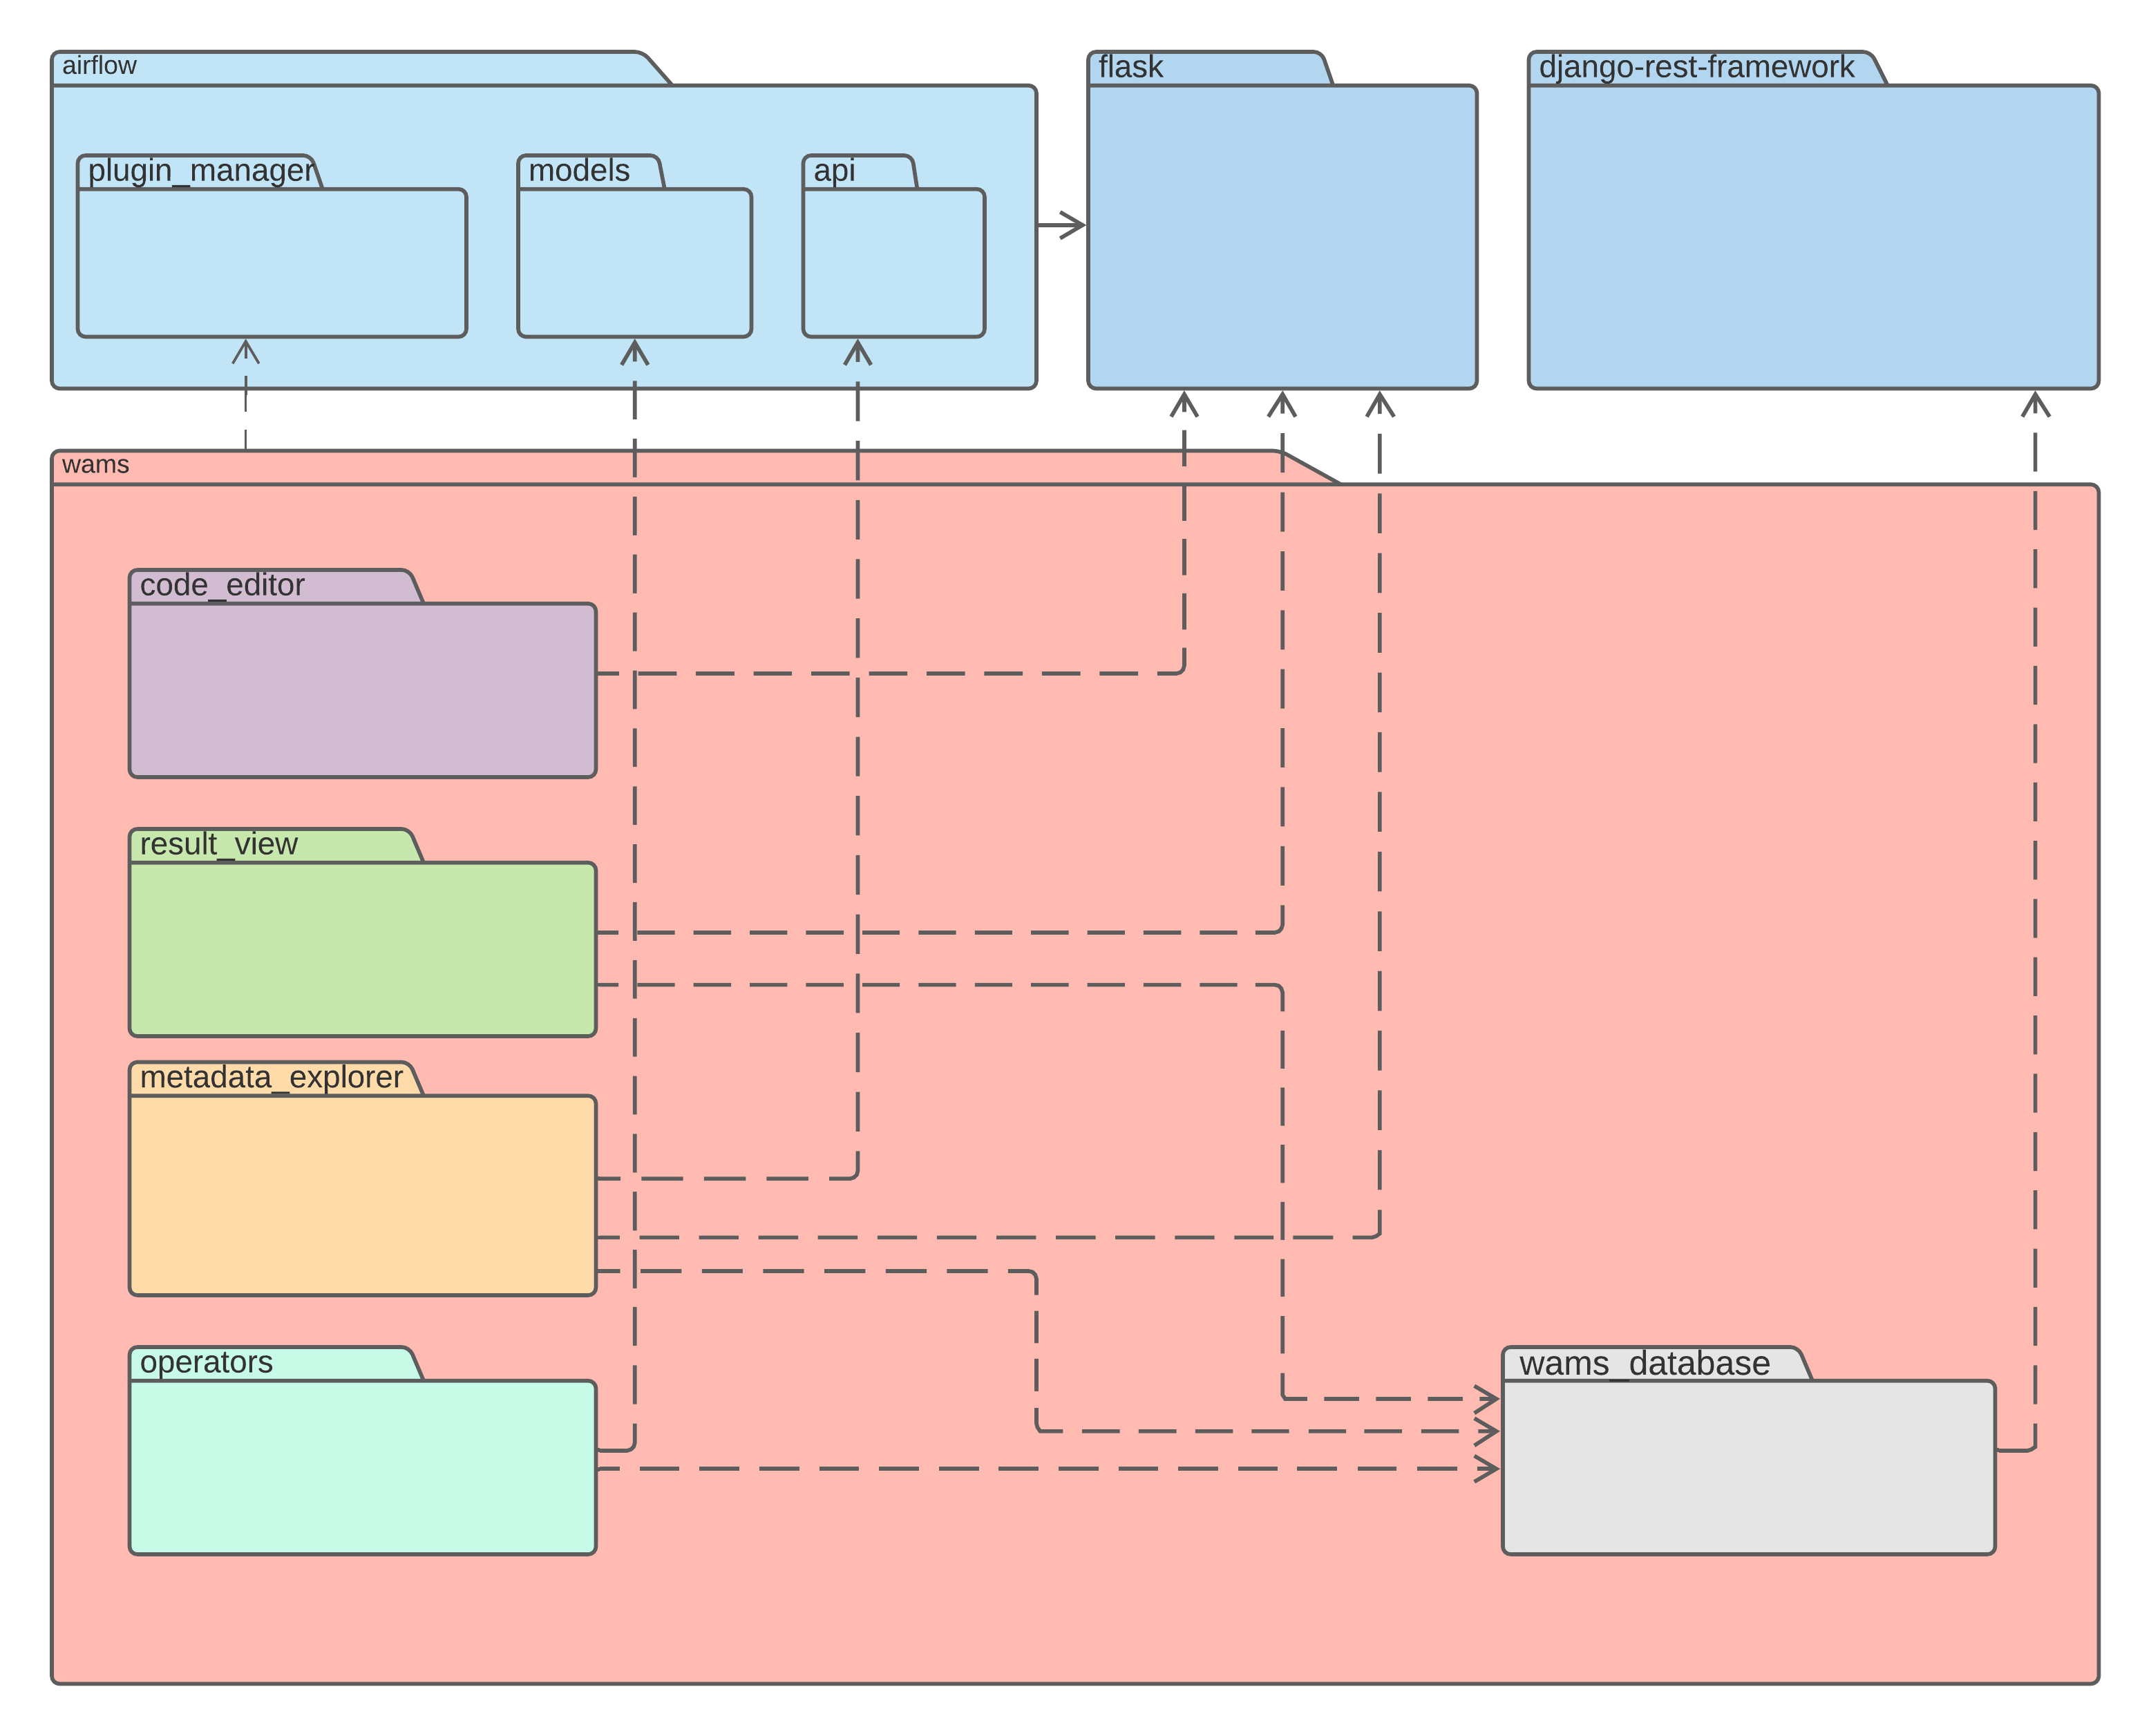
\includegraphics[width=\textwidth]{Diagramme/Paket.png}
    \caption{Paketdiagramm von WAMS}
    \label{fig:Paket}
\end{figure}

Diese Pakete werden in den nächsten Abschnitten einzeln behandelt.
Weiter greift WAMS auf mehrere Pakete innerhalb von Apache Airflow (\textit{airflow}) zu, insbesondere auf das Paket \textit{airflow.plugin\_manager} und auf das Paket \textit{airflow.api}. Das Paket \textit{airflow.plugin\_manager} liefert die Schnittstelle zur Einbindung des WAMS Plugins.
Das Paket \textit{airflow.api} enthält die Anwendungsprogrammierschnittstelle von Apache Airflow.

\subsection*{Code-Editor}
Der Code-Editor dient dazu den Python-Quellcode von Workflows in der Weboberfläche ändern zu können.
Hierbei wird das Airflow Plugin \gls{airflow-code-editor} von WAMS verwendet.

\subsection*{Result View}
Das Result View Paket erweitert die Weboberfläche von Airflow mit einem Tab zum Einsehen ausgewählter Ergebnisse und Zwischenergebnisse von Ausführungen von Workflows. 


\subsection*{Metadata Explorer}
Das Metadata Explorer Paket erweitert die Weboberfläche von Airflow durch einem Tab zum Einsehen der Metadaten einer Ausführung von Workflows. Die Metadaten werden über die Airflow API ermittelt.

\subsection*{Operators}
Das Operators Paket bündelt die in WAMS enthaltene Erweiterung der bereits in Apache Airflow existierenden Operatoren. 
In ihm sind Operatoren enthalten, die zu einer einfachen Anwendung von TGDS Workflows gedacht sind.
Außerdem ist ein Operator enthalten, der das Abspeichern von Ergebnissen und Zwischenergebnissen stark vereinfacht.

\subsection*{WAMSDatabase}
Das WAMSDatabase Paket ist zuständig für das Speichern von Daten im Zusammenhang mit Workflow-Instanzen.
\chapter{Design}
WAMS passt Airflow an die Bedürfnisse des Kunden an. WAMS liefert eine auf Experimente der Material- und Datenwissenschaften abgestimmte Konfiguration von Airflow, sowie zusätzlich benötigte Funktionalität in Form eines Airflow Plugins. Da die Webansicht von Airflow auf dem Flask Framework \gls{AppBuilder} basiert, bringt unser Plugin weitere Ansichten mit, die unter der Menüleiste eingefügt werden.

\section{Airflow Konfiguration}
\subsection{Nutzerverwaltung}
Airflow bietet standardmäßig fünf Nutzerklassen an auf die es alle Berechtigungen verteilt. Da WAMS nur drei Nutzerklassen hat, werden die Rechte wie folgt reduziert:
\begin{itemize}
    \item Admin: übernehmen die Rolle des \gls{Op} und erhalten für alle Bereiche
    Lese- und Schreibrechte. 
    \item Developer: erhalten Lese- und Schreibrechte für alle Bereiche, außer der Konfiguration von Airflow.
    \item Reviewer: erhält nur Leserechte.
\end{itemize}

Airflow übernimmt die Login-Seite von \gls{AppBuilder} und kann somit nach der Dokumentation von Flask \gls{AppBuilder} angepasst werden, um die Registrierung neuer
Nutzer anzubieten. Auch die neuen Ansichten, die von WAMS geliefert werden nutzen die 
Nutzerverwaltung von Flask \gls{AppBuilder}.

\section{Plugin}
Airflow bietet nativ noch nicht alle gewünschten Funktionalitäten. Daher bietet WAMS
noch drei weitere Ansichten um den gewünschten Funktionsumfang zu erreichen. Diese sind:
\begin{itemize}
    \item Editor-Ansicht: zum Editieren der DAG-Definitions-Dateien
    \item Result-Ansicht: zur Auflistung und Anzeigen der durch Workflows erstellte Dateien
    \item Metrics-Ansicht: zur Auflistung der ausgeführten Workflows-Instanzen 
    und den dazugehörigen Metadaten
\end{itemize}
Als zusätzliche Komponente bringt WAMS eine eigene Datenbank für die 
Speicherung der benutzerdefinierten Resultate und Zwischenergebnisse von Workflows-Instanzen und die dauerhafte Speicherung von Metadaten mit. Die Datenbank befindet sich in einem eigenen Container und kann von den anderen Ansichten über eine API angesprochen werden. %lebt? Sagt man das so?

\subsection{Editor-Ansicht}
Um das Editieren von Workflows in der Weboberfläche von Airflow zu ermöglichen, bedienen wir uns an dem bereits existierendem Plugin \gls{airflow-code-editor}. %Muss noch überarbeitet werden weiß nicht genau was wir da abgeändert haben
Dieses Plugin implementiert bereits eine Anzeige für die Ordnerstruktur und die Editierung von Textdateien in der Weboberfläche von Airflow.
Dabei nutzt es den Javascript Editor \gls{Codemirror}. Über die gewünschte Funktionalität hinaus bietet \gls{airflow-code-editor} zudem noch eine Git-Integration über die gleiche Weboberfläche an. %Diese Weboberfläche binden wir in unser Plugin ein, um dessen Funktionalität anzubieten. %wessen?


Um die Weboberfläche von \gls{airflow-code-editor} für unsere Anwendung zu nutzen, braucht es noch folgende Anpassungen:

\begin{itemize}
    \item Das Hauptverzeichnis wird von \verb!$AIRFLOW_HOME/! zu \verb!$AIRFLOW_HOME/dags/! geändert.
    \item In der Titelleiste von Airflow wird ein Reiter hinzugefügt, über den man auf die Weboberfläche des Plugins zugreifen kann.
    \item Die Zugriffsberechtigung auf die Weboberfläche muss von Admin auf Developer erweitert werden.
\end{itemize}

\subsection{Results-Ansicht}
Damit Nutzer von WAMS für einzelne Durchläufe eines Workflows jeweils Resultate abspeichern und über die Weboberfläche auf diese zugreifen können, bietet WAMS einen eigenen Operator (SaveResultsOperator) für die Speicherung von ausgewählten Dateien und eine weitere Webansicht für eine Ansicht der Ergebnisse.

\subsubsection{SaveResultsOperator}
Der Operator ist eine Unterklasse des BaseOperator von Airflow. Er nimmt als Argumente ein Verzeichnis, das er sichern soll oder eine Liste an Dateien, die gesichert werden sollen. Er kann am Schluss des Workflows ausgeführt werden, um ein Gesamtresultat zu speichern oder nach einzelnen Operatoren ausgeführt werden, um auch Zwischenresultate zu speichern.

Während seiner Ausführung baut er eine Verbindung mit der Datenbank von WAMS auf und legt die gewünschten Dateien in dieser ab. Der Operator übergibt der Datenbank neben den zu sichernden Dateien noch Informationen über den Workflow und der Workflow-Instanz, die den Operator ausführt, sodass die Datenbank die Dateien richtig zuordnen und eindeutig ablegen kann.


\subsubsection{Results-Webansicht}
Die Webansicht der erzeugten Ergebnisse wird mit Hilfe von Flask \gls{AppBuilder} erzeugt und enthält Komponenten, die die Workflows, Workflow-Instanzen und Workflowinstanzergebnisse aus der Datenbank abfragen und graphisch in der Weboberfläche darstellen können.


\subsection{Metadaten-Ansicht}
Da Airflow bereits eine API für den Zugriff auf Metadaten besitzt, wird die Metadaten-Ansicht von WAMS diese verwenden. 
Die Metadaten einer Workflowinstanz werden beim Löschen des zugehörigen Workflows oder beim Löschen der Workflowinstanz ebenfalls gelöscht. Um die Persistenz der Metadaten zu gewährleisten, werden die Metadaten einer Workflow-Instanz in der Datenbank von WAMS hinterlegt. Die Daten in der WAMS Datenbank sind dabei immutable und werden beim Löschen des Workflows nicht entfernt.

Die Aufgaben der Metadaten-Ansicht werden dabei wie folgt auf Klassen aufgeteilt:
Eine Klasse, die dafür zuständig ist, die Metadaten einer Worfklowinstanz, eine Liste von Instanzen eines Workflows und eine Liste von Workflows aus der WAMS-Datenbank zu holen. Diese Klasse hat dabei keinen Einfluss auf die GUI.
Zwei Klassen, die gemeinsam mit dem Flask-Blueprint dieser Ansicht für die graphische Darstellung der Workflows, Workflow-Instanzen und Metadaten verantwortlich sind. Eine Klasse ist dabei dafür zuständig, die Metadaten, welche als .json Datei vorliegen, graphisch darzustellen.

\subsection{WAMS-Datenbank}
Airflow nutzt bereits eine Datenbank für die Speicherung der Metadaten der Ausführungen von Workflows. Folgende Beschränkungen führen dazu, dass die Datenbank nicht ohne Anpassung von WAMS übernommen werden kann:
\begin{itemize}
    \item Die Metadaten gelöschter Workflows werden nicht erhalten.
    \item Es gibt keine Möglichkeit Dateien als Resultat von Workflows zu sichern.
\end{itemize}

Somit dient die WAMS-Datenbank sowohl als ein Speicher für die Ergebnisse und Zwischenergebnissen von Workflow-Ausführungen als auch eine Erweiterung der Airflow-Datenbank. Die WAMS-Datenbank wird Über eine API-Klasse, die POST- und GET-Methoden anbietet, angesprochen. Diese Klasse trifft abhängig von der Anfrage die Entscheidung, ob Metadaten oder Resultate einer Workflow-Instanz angefragt werden und delegiert die Beschaffung an andere Klassen.

Wird eine Datei angefordert, die Ergebnis einer Workflow-Instanz war, wird diese Anfrage an
die ResultHandler-Klasse weitergeleitet. Die ResultHandler-Klasse speichert die Ergebnisse
nach der dazugehörigen Workflow-Instanz in einem Verzeichnis und beschafft diese auf
Anfrage. Dabei werden gleichzeitig die Metadaten für die ausführende Workflow-Instanz
in einer MySQL-Datenbank gespeichert.

Wird eine Anfrage nach Metadaten zu einer Workflow-Instanz gestellt, wird diese 
MetricsGetter weitergeleitet. MetricsGetter versucht zunächst eine Anfrage über die
Airflow-Datenbank aufzulösen. Falls diese Anfrage jedoch erfolglos war, wird eine weitere
Anfrage an die eigene MySQL-Datenbank gestellt. Somit besteht auch nach Löschung eines 
Workflows die Möglichkeit auf Metadaten gelöschter Workflows zuzugreifen. Somit ist das Prinzip der Transparenz eingehalten, da für den Anwender nicht ersichtlich ist, aus welcher Datenbank die Informationen und Ergebnisse stammen, aber auch sichergestellt wird, dass immer die aktuellsten und korrekte Ergebnisse geliefert werden.
\chapter{Klassenbeschreibung}

\begin{figure}[ht]
    \centering
    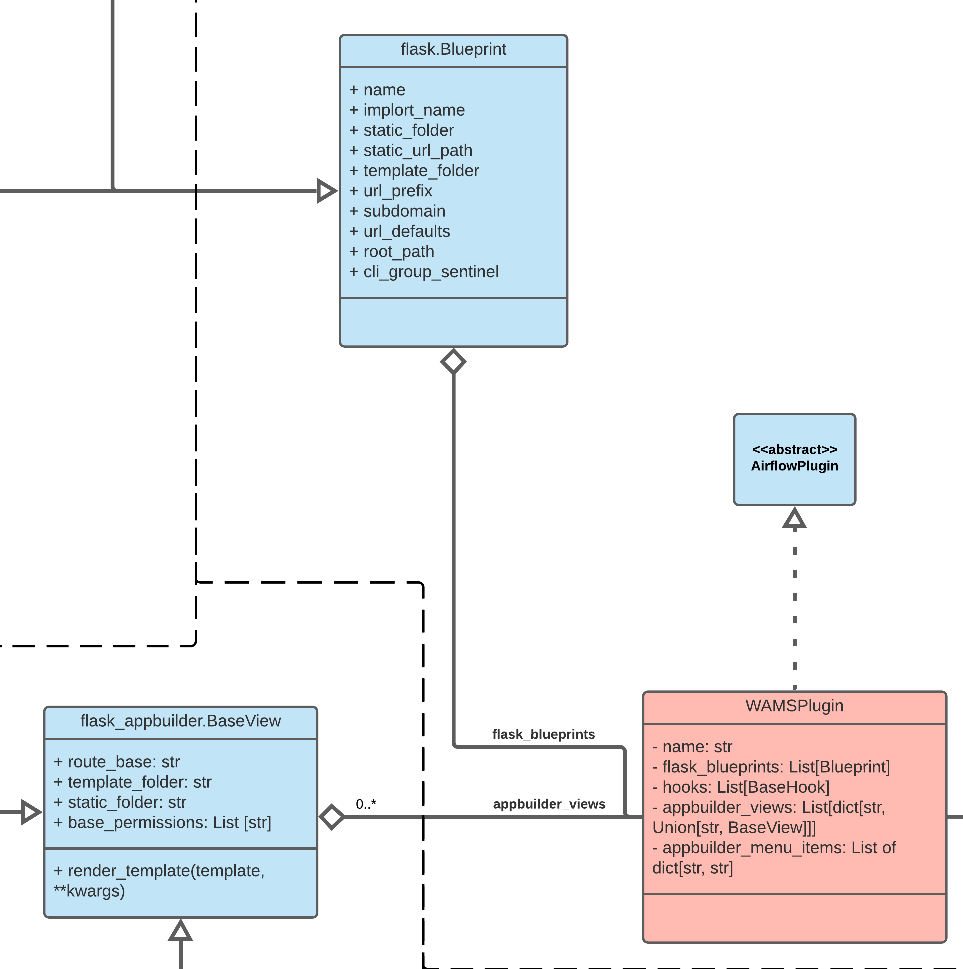
\includegraphics[width=\textwidth]{Diagramme/KlassendiagrammAusschnitte/Klassendiagramm - wamsplugin.png}
    \caption{Wams package}
    \label{fig:WamsPlugin}
\end{figure}

\subsection{WAMSPlugin}
Main Class of the WAMS Plugin for Airflow. Ties together the new views, functions and operators added in the plugin and implements the AirflowPlugin interface.
%Wrapper Klasse die die Hauptlogik des Plugins enthält und das AirflowPlugin interface implementiert.

\subsection{WAMSConfig}
Utility class that holds a dictionary of key value pairs, that represent the configuration of
WAMS. By default it loads the configuration stored in \verb!default_config.yaml!. An Config
singelton object is created during the initialisation of the application and its values are 
accessed via getter and setter methods to validate the inputs.
%Config datei siehe Daniel

\section{code\_editor}
\begin{figure} [ht]
    \centering
    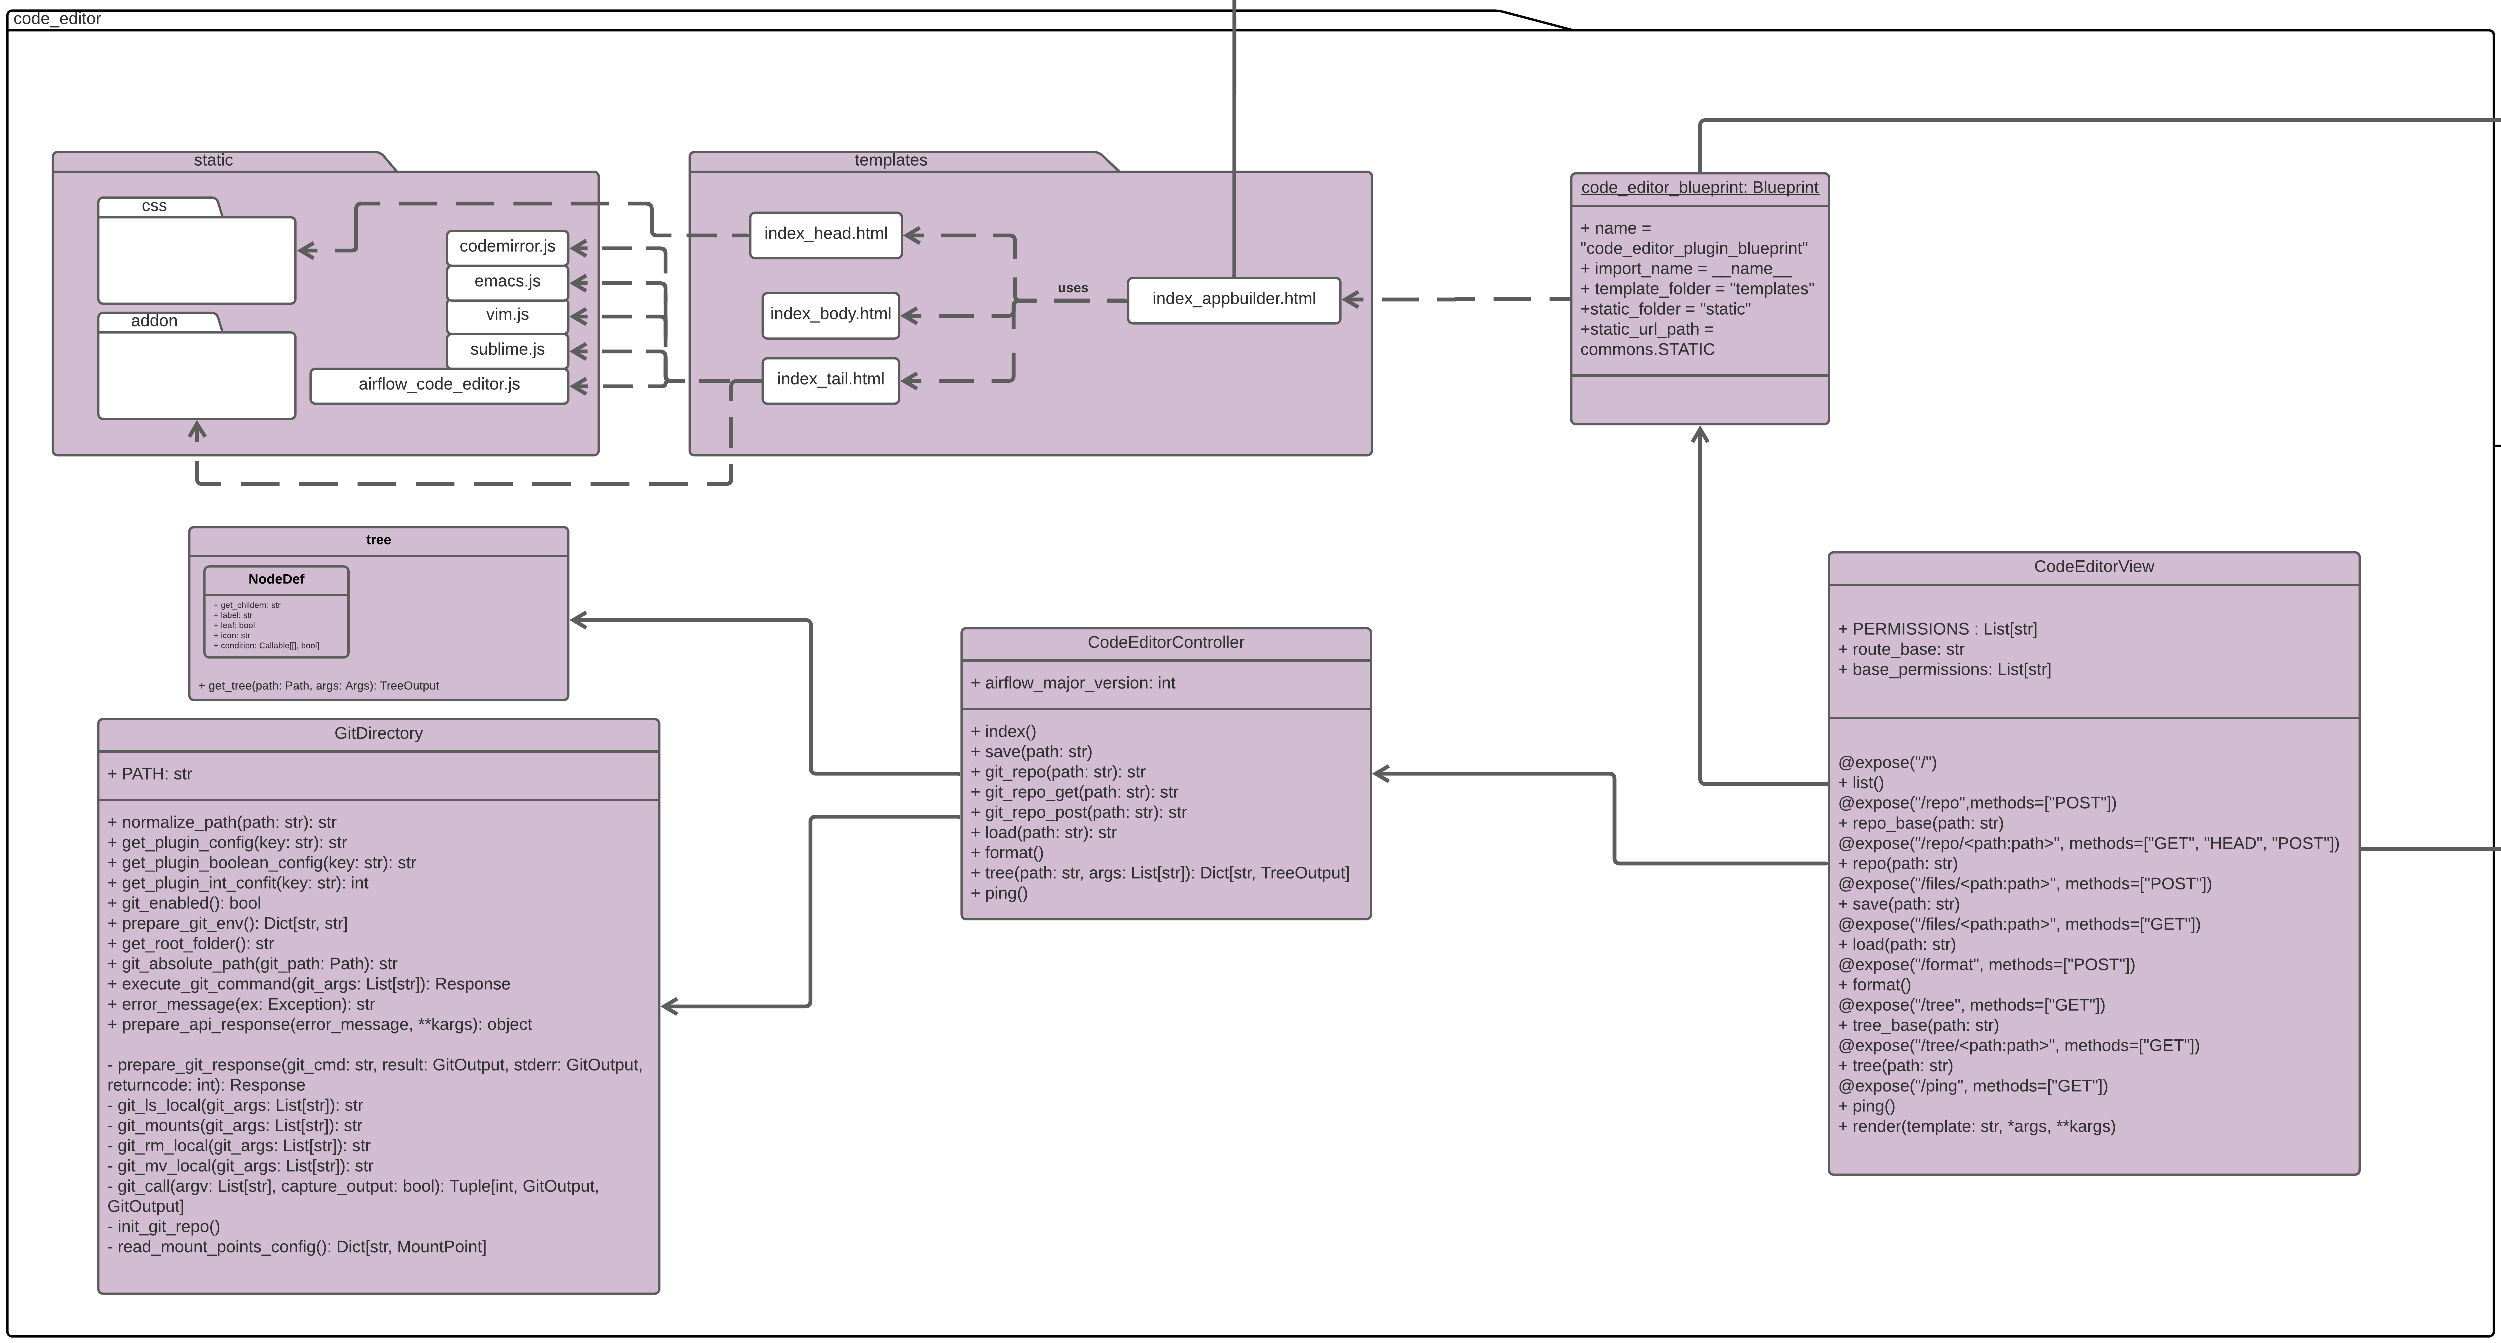
\includegraphics[width= \textwidth]{Diagramme/KlassendiagrammAusschnitte/Klassendiagramm -codeEditor.png}
    \caption{CodeEditor package}
    \label{fig:codeEditor section}
\end{figure}

\subsection{CodeEditorView}
Extends the flask\_appbuilder.BaseView class and handles the frontend of the CodeEditor package.
The CodeEditor view is added according to the Flask-AppBuilder Framework, that is used by Airflow for its Web-UI. It restricts access to the Editor according to the permissions and exposes the necessary URL-paths.

\subsection{CodeEditorController}
Implements the necessary logic for CodeEditorView and fetches the required data from GitDirectory, 
Tree.py and the dags directory.  

\subsection{code\_editor\_blueprint:Blueprint}
Flask blueprint used to handle the look and feel of the CodeEditor view.

\subsection{GitDirectroy}
Initializes and manages the git repository of the \verb!dags! folder. It
provides various methods to execute specific git commands on the git repository. 

\subsection{code\_editor.templates}
Templates folder for the code\_editor\_blueprint containing HTML files that determine the look of the CodeEditor view.

\subsection{code\_editor.static}
Static folder for the code\_editor\_blueprint containing CSS and JS files that determine the look and 
behavior of the CodeEditor view. It contains the files necessary for CodeMirror, directory and git view.

\subsection{tree}
Utility-class that is used by CodeEditorController to represent a file tree or git directory.


\subsection{results\_view\_blueprint:Blueprint}
Flask blueprint used to handle the look and feel of the Results view.


\section{metrics\_explorer}
Damit Nutzer von Airflow eine Übersicht über Metadaten von allen bereits ausgeführten Workflow Instanzen haben, fügt WAMS eine weitere Ansicht dafür hinzu.

 \begin{figure} [ht]
    \centering
    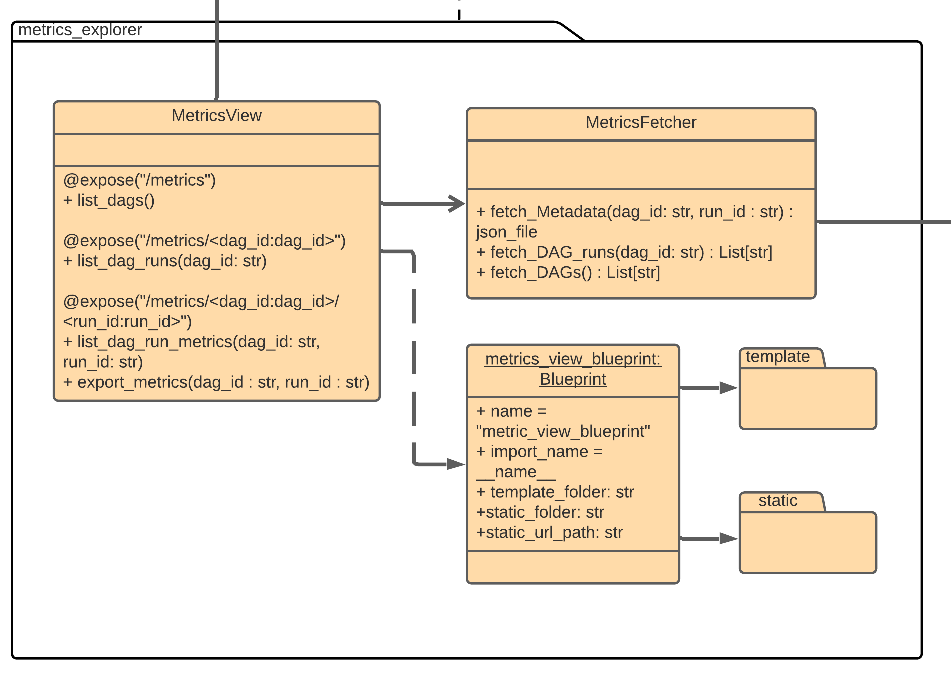
\includegraphics[width=\textwidth]{Diagramme/KlassendiagrammAusschnitte/Klassendiagramm -metadata explorer.png}
    \caption{Metadata package}
    \label{fig:metadata section}
\end{figure}


\subsection{MetricsView}
Extends flask\_appbuiler.BaseView to add a new view to the Webinterface of Airflow. It manages the
access rights and the frontend of the Metrics view.
%to write

\subsubsection{+ list\_dags()}
Lists all workflows in the current Airflow instance so that the user can select one of them.
The MetricsView gets the list from a MetricsFetcher instance.
\subsubsection{+ list\_dag\_runs(dag\_id: str)}
Lists all instances of a workflow that was just selected so that the user can select one of them.
It gets its the list from a MetricsFetcher instance.
\subsubsection{+ list\_dag\_run\_metrics(dag\_id: str, run\_id: str)}
Displays the metadata of the selected workflow instance.
It gets the metadata in form of a Json file from a MetricsFetcher instance.

\subsection{MetricsFetcher}
Fetches the required data for MetricsView from the WAMS Database. It converts the specific 
requests from MetricsView into API calls.

\subsubsection{+ fetchMetadata(dag\_id: str, run\_id) : json\_file}
Creates a json file from the response of the WAMS Database api calls and returns the that file.

%
%\subsection{JsonView}
%Responsible for formatting JSON files that are generated by MetricsFetcher. 

%\subsubsection{+ <<create>> \_\_init\_\_(file: json\_file)}
%Creates a new JsonView 

%\subsubsection{+ results(): json}
%Formats a JSON file making sure that the metadata is consistantly displayed.

%\subsubsection{+ download\_file()}
%Triggers the download of the formated JSON file.
%

\subsection{metrics\_view\_blueprint:Blueprint}
Flask blueprint that specifies the files used to handle the look and feel of the Metrics view.

\subsection{metrics\_explorer.templates}
Templates folder for the metrics\_view\_blueprint containing HTML files that determine the look of Metrics view.


\subsection{metrics\_explorer.static}
Static folder for the code\_editor\_blueprint containing CSS and JS files that determine the look 
and behavior of the Metrics view.

\section{wams\_operators}
\begin{figure} [ht]
    \centering
    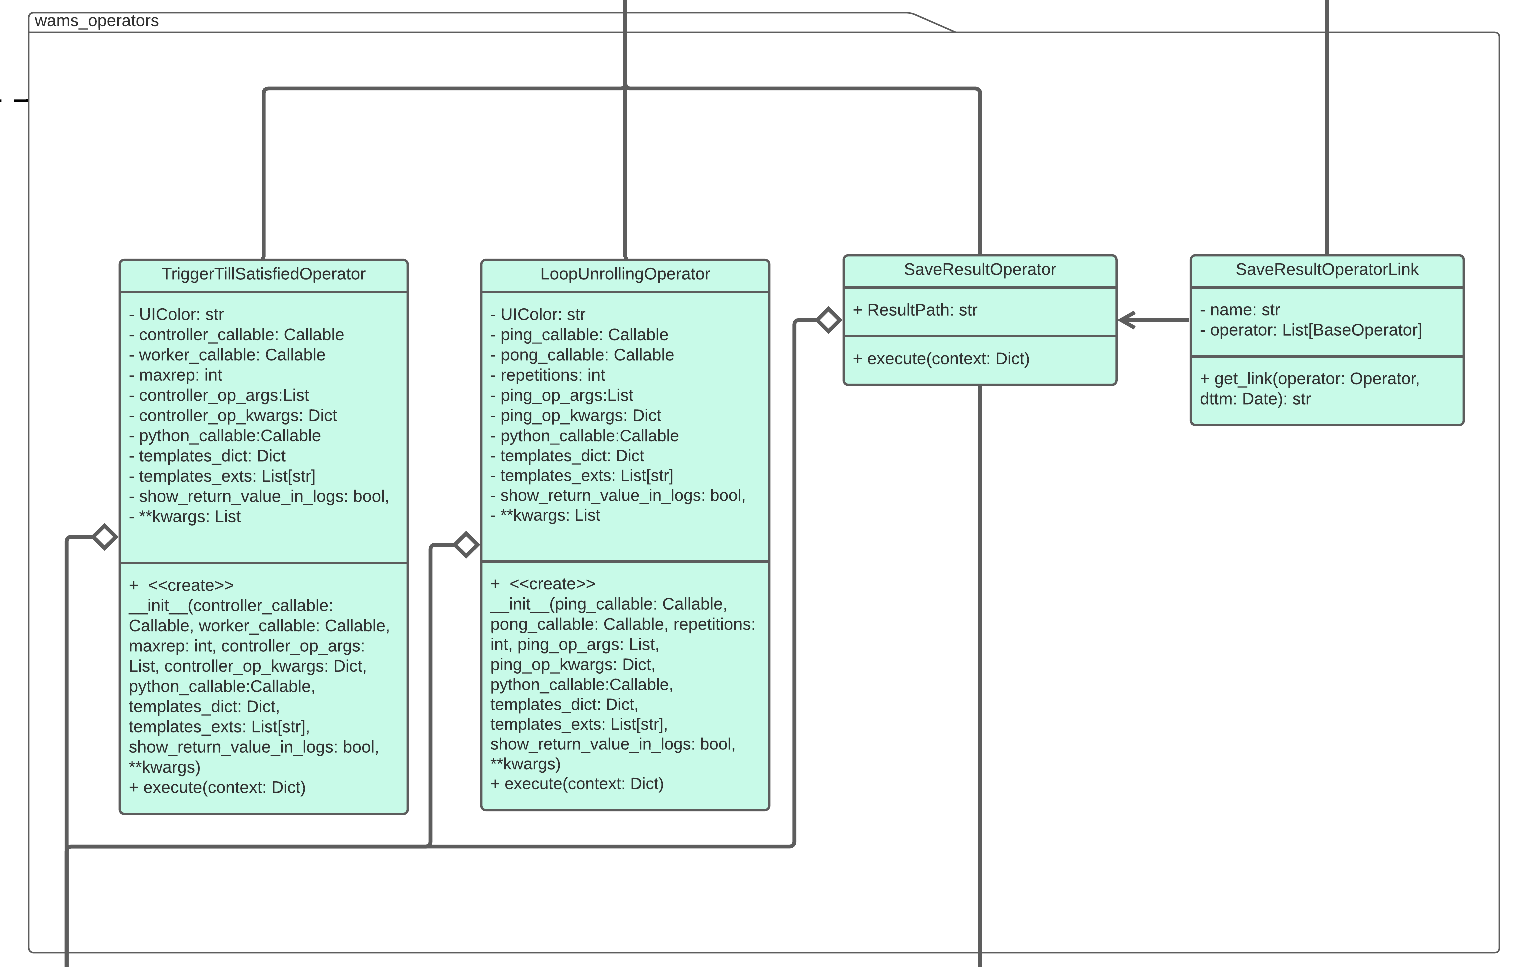
\includegraphics[width = \textwidth]{Diagramme/KlassendiagrammAusschnitte/Klassendiagramm -operators.png}
    \caption{Oparators package}
    \label{fig:operators section}
\end{figure}

\subsection{LoopUnrollingOperator}
%Operator class used for dynamically created tasks like the theory guided maschine learning modell.
This class represents an operator for Apache airflow and inherits from its base operator class.
The LoopUnrollingOperator receives two python callables. It executes both of them alternating as often as specified in the repetition parameter of its \textit{\_\_init\_\_()} method. The results of the callables can be used as input parameters for each repetition to allow to increase the accuracy of the model. The first callable can be started with parameters also passed via the \textit{\_\_init\_\_()} method.

\subsubsection{+  \_\_init\_\_(ping\_callable: Callable, pong\_callable: Callable, repetitions: int, ping\_op\_args: List, ping\_op\_kwargs: Dict, python\_callable:Callable, templates\_dict: Dict, templates\_exts: List[str], show\_return\_value\_in\_logs: bool, **kwargs: Dict)}

This method configures an instance of the LoopUnrollingOperator. In the parameters both callables and the number of repetitions must be parsed. Optional arguments like input parameters for the first callable execution can also be parsed.

\subsubsection{execute(context: Dict)} 
This method is derived from Airflows \textit{BaseOperator}-class. It initiates the execution of the task represented by the LoopUnrollingOperator.


\subsection{TriggerTillSatisfiedOperator}
This class represents an operator for Apache Airflow and inherits from its base operator class.
The TriggerTillSatisfiedOperator receives two python callables. In opposition to the \textit{LoopUnrollingOperator} the number of repetitions is not set via the \textit{\_\_init\_\_()} method but can change dynamically. The controller callable triggers the worker callable every time the worker has finished its work until the controller is satisfied with the result. To prevent to long runs a maximum of repetitions can also be passed in the \textit{\_\_init\_\_()} method. The controller callable receives the return values of the worker after every run of the worker.

\subsubsection{\_\_init\_\_(controller\_callable: Callable, worker\_callable: Callable, maxrep: int, controller\_op\_args: List, controller\_op\_kwargs: Dict, python\_callable:Callable,
templates\_dict: Dict, templates\_exts: List[str], show\_return\_value\_in\_logs: bool, **kwargs: Dict)}
This method configures an instance of the TriggerTillSatisfiedOperator. In the parameters the controller and worker callables must be parsed. Optional arguments like the maximum number of repetitions and input parameters for the controller can also be parsed.

\subsubsection{execute(context: Dict)} 
This method is derived from Airflows \textit{BaseOperator}-class. It initiates the execution of the task represented by the TriggerTillSatisfiedOperator.

\subsection{SaveResultOpertator}
This class represents an operator for Apache Airflow and inherits from its base operator class.
The main purpose of the SaveResultOperator is making the process of saving results, interim 
results and metadata as easy and uncomplicated as possible. The developer of a workflow should be able to save
results, interim results and metadata of his workflow by only adding this operator after a previous task 
which produced the result. The final storage control is not a part of this class but of the 
\textit{wams\_database} package.

\subsubsection{+ execute(context: Dict)} 
This method is derived from Airflows \textit{BaseOperator}-class. It saves the result or interim result of the workflow the SaveResultOperator belongs to in the current state of the workflow execution. 

\subsection{SaveResultOperatorLink}
This class creates a link which is added to every \textit{SaveResultOperator}. The link will be shown in the menu that pops up if the operator is clicked after a workflow was run. The link leads to the result view for the interim result or result stored by the \textit{SaveResultOperator} the SaveResultOperatorLink belongs to.

\subsubsection{+ get\_link(operator: Operator,  dttm: Date): str}
This method receives the operator the link for should be shown in and the date and time of its execution and returns a link. The operator should be a \textit{SaveResultOperator} and the link should lead directly to the result view for the result or interim result stored by this specific \textit{SaveResultOperator}.

\begin{figure} [h]
    \centering
    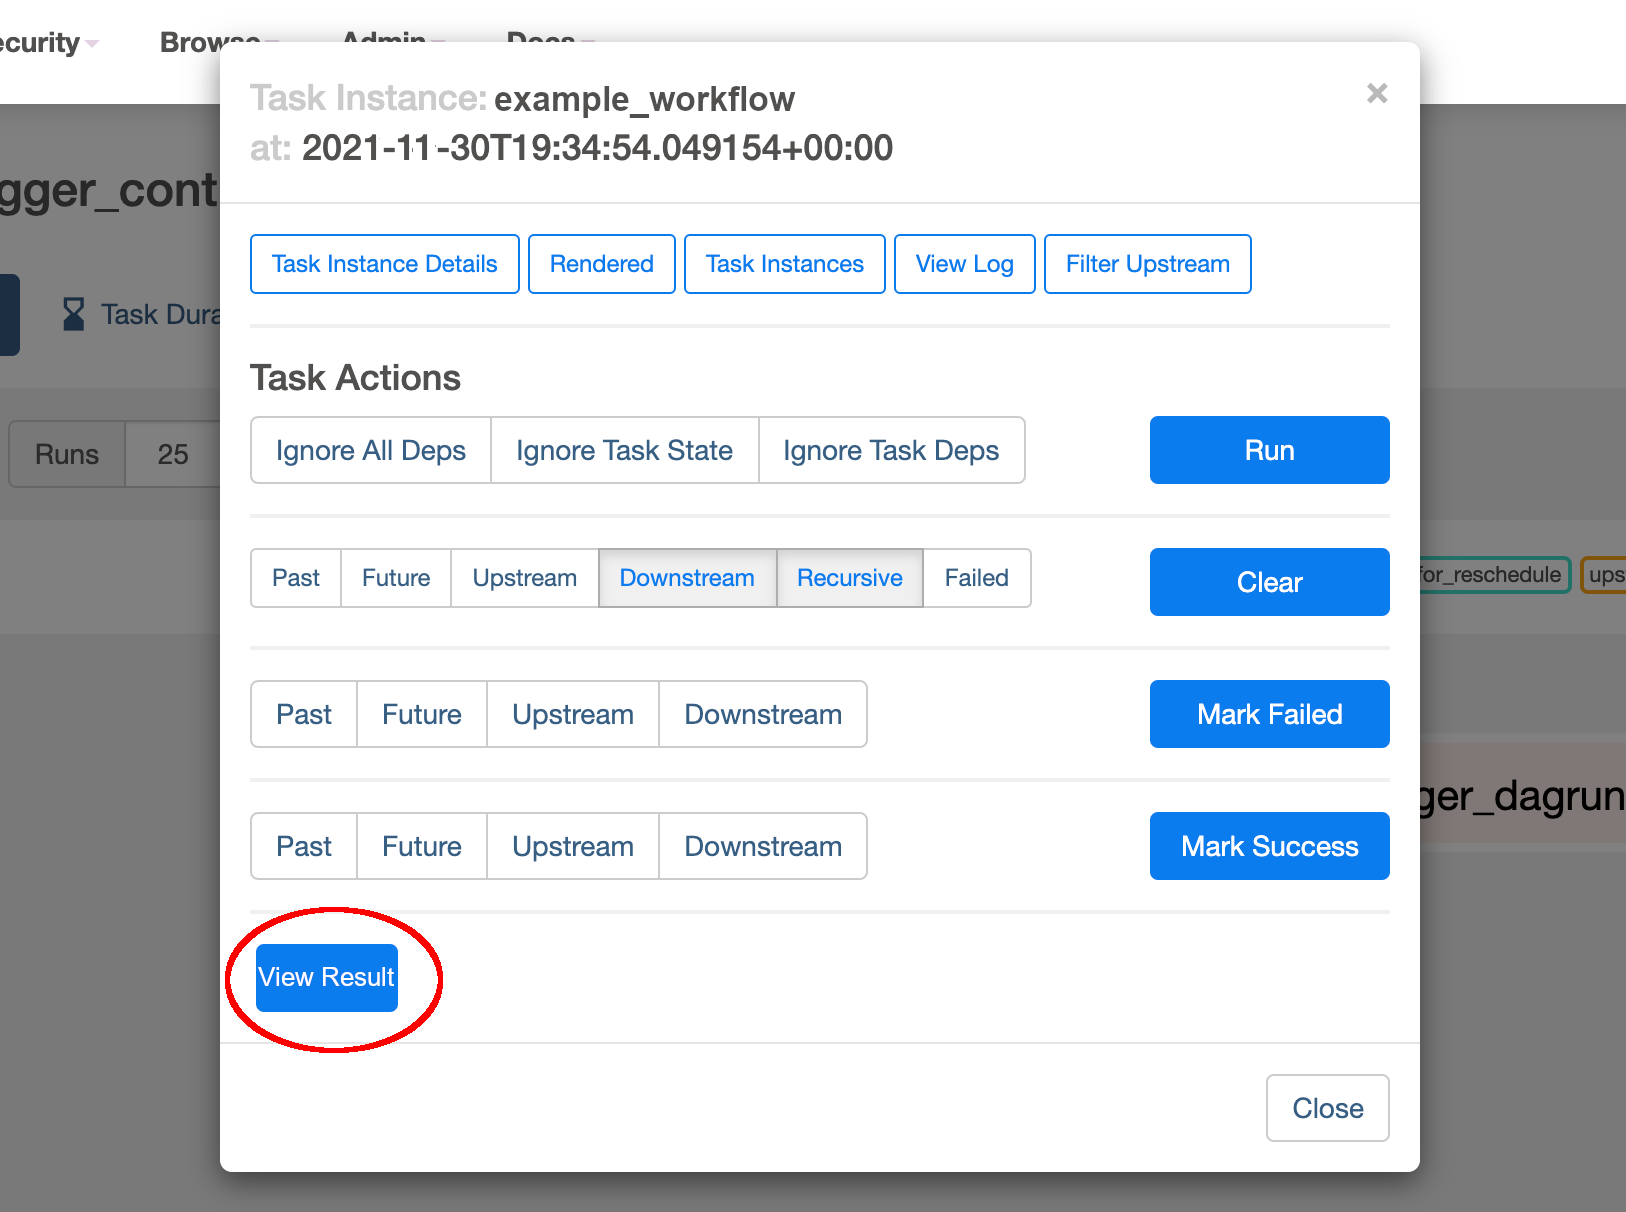
\includegraphics[width = 0.75\textwidth]{Grafiken/operator_extra_link.png}
    \caption{Beispielhafte Ansicht der Weboberfläche, wenn nach der Ausführung des Workflows \textit{example\_workflow} der SaveResultOperator angeklickt wurde. Die Klasse SaveResultOperatorLink sorgt dafür, dass der rot eingekreiste Button hinzugefügt wird}
    \label{fig:expSaveLink}
\end{figure}

\section{wams\_database}
Airflow bietet schon eine Datenbank, Metadaten bezüglich der einzelnen Workflows und den
ausgeführten Workflow Instanzen bietet. Jedoch bietet Airflow keine eigene Datenbank, die die
Ergebnisse von Workflows speichert. Um diese Funktionalität zu implementieren, hat WAMS eine
eigene Datenbank in einem separatem Container, die die Resultate, die über den SaveResultOperator gespeichert werden, speichert. %%%%%%TODO

\begin{figure} [ht]
    \centering
    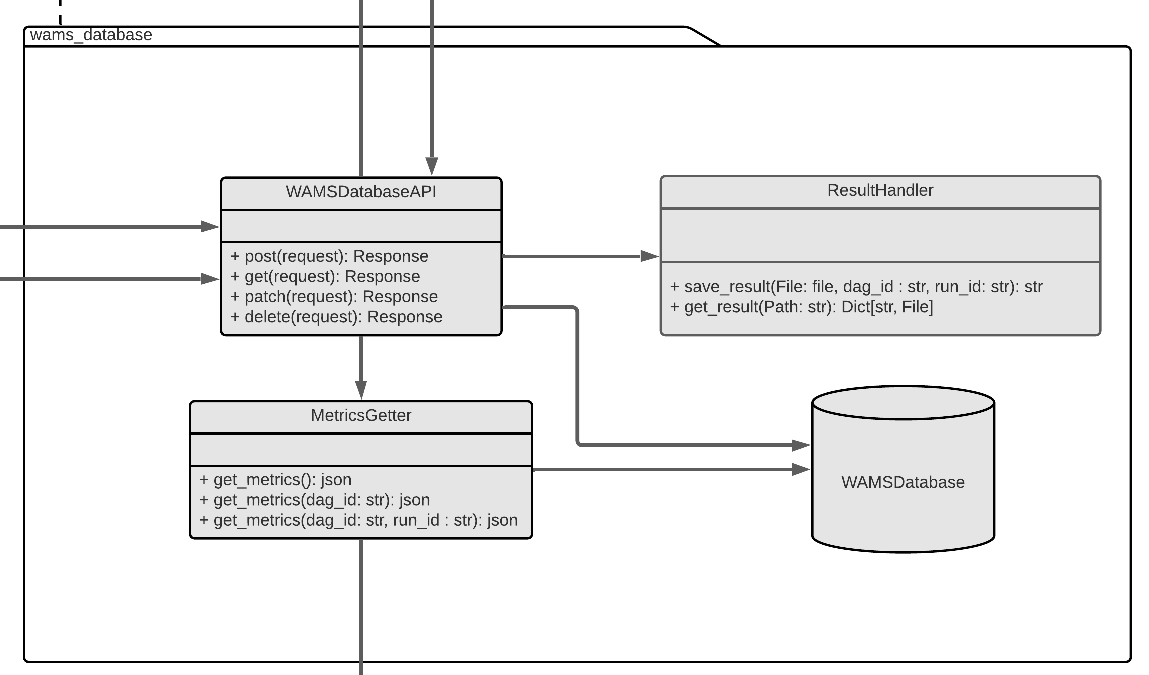
\includegraphics[width=0.9\textwidth]{Diagramme/KlassendiagrammAusschnitte/Klassendiagramm -database.png}
    \caption{Database package}
    \label{fig:database section}
\end{figure}

\subsection{WAMSDatabaseAPI}
Extends the rest\_framework.views.APIView to provide an API Django REST API for the other
parts of the WAMS-Plugin. The functions that this API handels are:
\begin{itemize}
    \item List all existing workflows and workflow instances
    \item Fetch the metadate for a particular workflow instance
    \item Upload a file generated by a workflow instance for persistent storage
    \item Fetch a file generated by a workflow instance to display it to the user
\end{itemize}
The WAMSDatabaseAPI class recognizes which action is requested and forwards the action to
the ResultHandler or MetricsGetter.

\subsubsection{+ post(request): Response}
Implementation of the POST endpoint of the Django RESTful API. This handles inserting new data into the WAMSDatabase and returns a response object depending on the outcome of the operation.
%Handles a POST request made to the API this class represents. 
\subsubsection{+ get(request): Response}
Implementation of the GET endpoint of the Django RESTful API. This handles getting data from the WAMSDatabase and returns a response object depending on the outcome of the operation.
%Handles a GET request made to the API this class represents.
\subsubsection{+ patch(request): Response}
Implementation of the PATCH endpoint of the Django RESTful API. This handles overwriting data within the WAMSDatabase and returns a response object depending on the outcome of the operation.
\subsubsection{+ delete(request): Response}
Implementation of the DELETE endpoint of the Django RESTful API. This handles removing data within the WAMSDatabase and returns a response object depending on the outcome of the operation.

\subsection{ResultHandler}
Handles the results generated by a workflow instance, that are uploaded via the
SaveResultOperator. Each file uploaded is stored in a directory according to the workflow
and the workflow instance that generated it.

\subsubsection{+ save\_result(File: file, dag\_id: str, run\_id: str): str}
Saves a given file in the results directory according to the dag\_id and run\_id so that they can
be retrieved for later use.
\subsubsection{+ get\_result(Path: str): Dict[str, File]}
Retrieves the results from a DAG run from the results directory according to the given path.


\subsection{MetricsGetter}
Handles the metadata generated by airflow for a workflow instance. When the metadata for a
workflow instance is requested it firstly polls the Airflow database over the Airflow API
for its data, if no data is found, it polls the WAMSDatabase for the data, since the workflow
might have been deleted.

\subsubsection{+ get\_metrics(): json}
Makes an API call to get a list of all workflows in airflow.

\subsubsection{+ get\_metrics(dag\_id: str): json}
Makes an API call to get a list of all workflow instances of a given workflow.

\subsubsection{+ get\_metrics(dag\_id: str, run\_id : str): json}
Makes an API call to get the metadata for a specific workflow instance.


\subsection{WAMSDatabase}
MySQL Database that persistently stores the results, interim results and the metadata for a workflow instance. After a workflow finishes and stores its results its metadata is fetched from the Airflow database and stored in this database to protect it from deletion after a workflow is deleted.
Results and interim results are stored into the database by the \textit{SaveResultOperator}.
%PPPPPaRamEteR spEiCherN?

\section{result\_view}

\begin{figure} [ht]
    \centering
    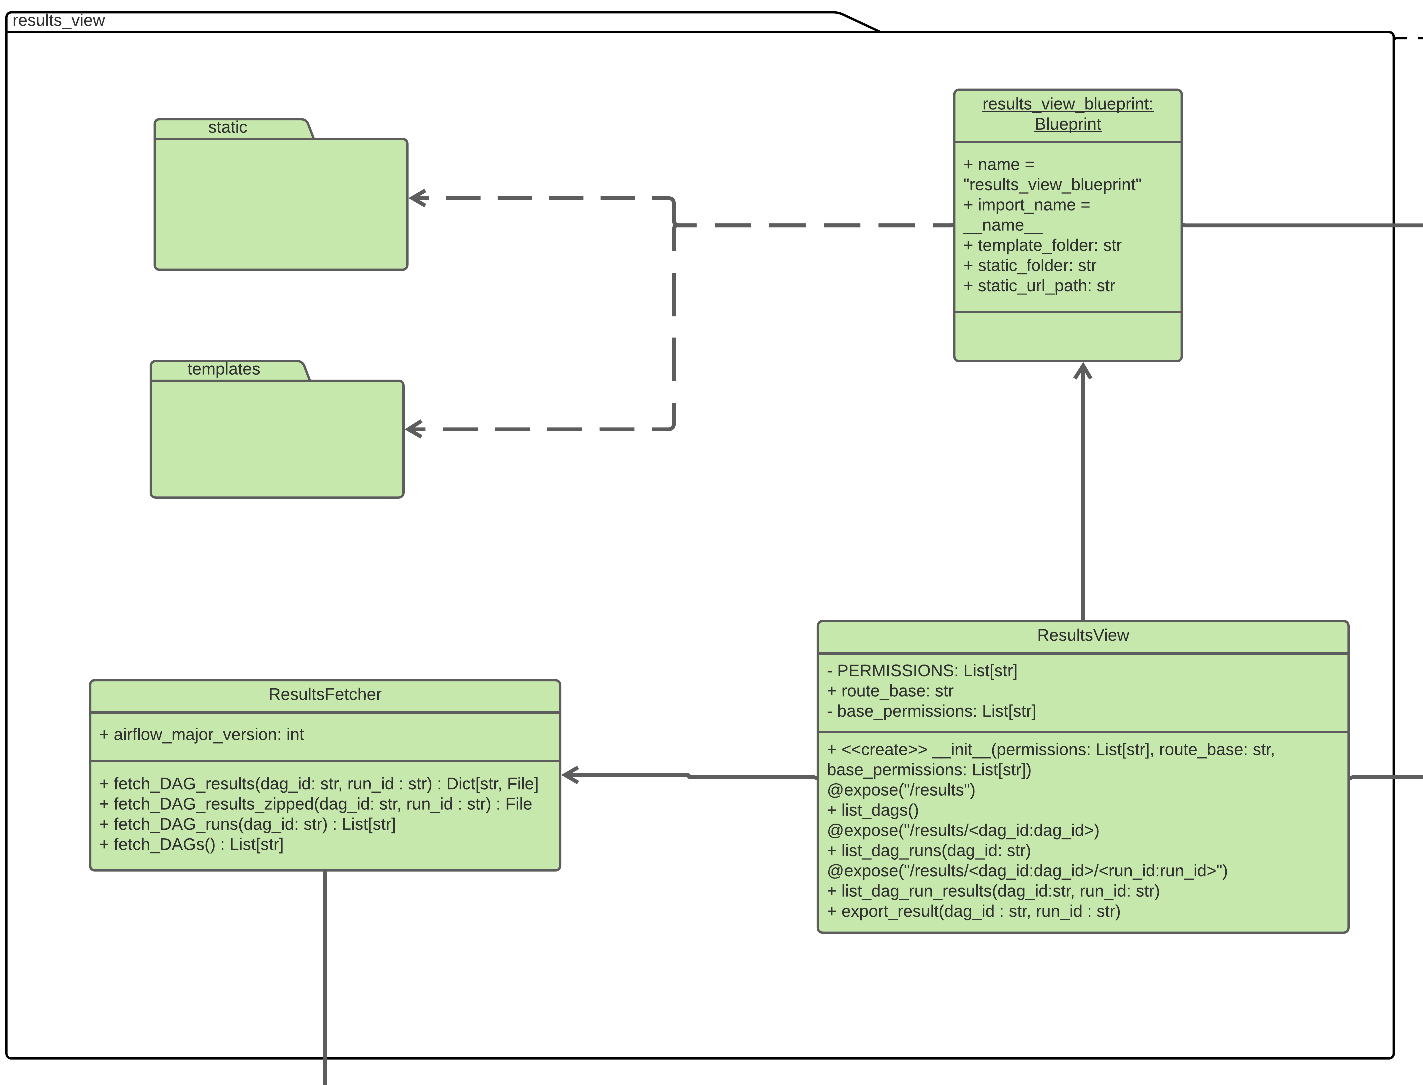
\includegraphics[width = \textwidth]{Diagramme/KlassendiagrammAusschnitte/Klassendiagramm -results view.png}
    \caption{Result\_view package}
    \label{fig:results section}
\end{figure}

\subsection{ResultsView}
Frontend for a AppBuilder view that lists all results generated and stored with the SaveResultOperator in the WAMSDatabase by the workflow and workflow instance that generated them.

\subsubsection{+ \_\_init\_\_(permissions: List[str], route\_base: str, base\_permissions: List[str]}
Creates a new ResultsView instance.

\subsection{+ list\_dags()}
Lists all workflows in the current Airflow instance so that the user can select one of them.
The ResultsView gets the list from a ResultsFetcher instance.

\subsubsection{+ list\_dag\_runs(dag\_id: str)}
Lists all instances of a workflow that was just selected so that the user can select one of them.
It gets its the list from a ResultsFetcher instance.

\subsubsection{+ list\_dag\_run\_results(dag\_id:str, run\_id: str)}
Displays the results of the selected workflow instance.
It gets the results from a ResultFetcher instance.

\subsubsection{+ export\_result(dag\_id : str, run\_id : str)}
Triggers the export of the results of a workflow instance.



\subsection{results\_view\_blueprint:Blueprint}
Flask blueprint used to handle the look and feel of the Results view.

\subsection{ResultsFetcher}
Backend for Results view that requests the required data from the WAMS Database over the network,
with the needed REST API calls.

\subsubsection{+ fetch\_DAG\_results(dag\_id: str, run\_id : str) : Dict[str, File]}
Constructs an API call to the WAMS Database that gets a list of all the files created by a 
given workflow instance.

\subsubsection{+ fetch\_DAG\_runs(dag\_id: str) : List[str]}
Constructs an API call to the WAMS Database that gets a list of all workflow instances that were created from a given workflow.

\subsubsection{+ fetch\_DAGs() : List[str]}
Constructs an API call to the WAMS Database that gets a list of all workflows in the Airflow database.

\subsection{result\_view.static}
Templates folder for the metrics\_view\_blueprint containing CSS and JS files that determine
the look and behavior of the Results view.

\subsection{result\_view.templates}
Templates folder for the metrics\_view\_blueprint containing HTML files that determine the 
look of the Results view.

\section{Externe Klassen} 
Klassen die nicht im Rahmen des Projekts entwickelt werden, aber trotzdem für den Aufbau relevant 
sind, da sie erweitert werden oder referenziert werden.

\subsection{AirflowPlugin}
Specifies the fields a plugin class must assign values to making Airflow able to import the Plugin.

\subsection{flask\_appbuilder.BaseView}
Base class from the Flask Appbuilder that declares the behaviour of a website created by Flask AppBuilder.

\subsection{BaseOperator}
Base class for workflow operators, that are then used in a workflow to be executed by the
Airflow worker.

\subsection{BaseOperatorLink}
Base class for classes that add a link to a workflow operator task page.

\subsection{Airflow API}
The REST API that Airflow exposes to access the various functions of the Airflow CLI. It also grants access to the metadata for workflow instances.

\subsection{List DAGs (resource)}
A list of all workflows in Airflow.

\subsection{List DAG runs (resource)}
A list of all workflow instances in Airflow.

\subsection{flask.Blueprint}
Class that specifies Flask which directories are to be used to specify the look and feel of a Website.

\subsection{appbuilder/general/model/list.html}
A HTML template from the Flask AppBuilder Framework.

\subsection{rest\_framework.views.APIView}
The base class for a Django REST API that handles the requests via its own implementation of pre-defined methods.


\include{Kapitel/Abläufe}
\include{Kapitel/Änderungen zum pflichtenheft}
%\chapter{Anhang}
\blindtext
\printglossary
%Exportieren von Dag definition files über Applikation exportieren
%Braucht man um Workflow Instanzen sowie Workflows zu erportieren
\end{document}

%PRIO1
%Hochladen von Dateien (Config)
%Dateiexplorer und Festlegen von Orten für Ergebnisse

%PRIO2 TODO
%Liveanzeige von Logdateien